\documentclass[a4paper,12pt]{article}
\usepackage[a4paper, hmargin={1.5cm,1.5cm}, vmargin={1.5cm,1.5cm}]{geometry}
\usepackage{amsmath}
\usepackage{amsthm}
\usepackage{amsfonts}
\usepackage{color}
\usepackage[final]{graphicx}
\usepackage{subcaption}
\usepackage{wrapfig}
\newtheorem{remark}{Remark}[]
\newtheorem{prop}{Proposition}
\usepackage{amssymb}

\newcommand{\R}{\mathbb{R}}
\newcommand{\C}{\mathbb{C}}
\newcommand{\N}{\mathbb{N}}
\newcommand{\Q}{\mathbb{Q}}
\newcommand{\Lagr}{\mathcal{L}}


% Title Page
\title{Poisson Problem in 2D\\with Modified Cassini Egg Domain}
\author{Alifian Mahardhika Maulana}


\begin{document}
\maketitle
\section{Poisson Problem}
\subsection{Strong Form}
\begin{figure}[h!]
	\centering
	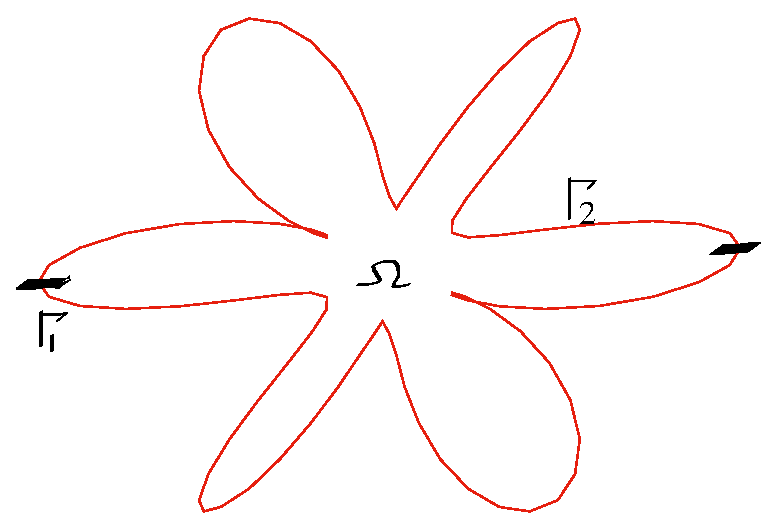
\includegraphics[width=0.5\linewidth]{picture/boundary}
	\caption{Modified Cassini Egg Domain}
	\label{fig:domain}
\end{figure}
Let's consider $f:\Omega \rightarrow \R$ and $g:\Gamma \rightarrow \R$ be given.\\
Then we define Poisson Problem, Find $u:\Omega \rightarrow \R$ s.t.
\begin{equation}\label{eq:poisson}
\begin{cases}
-\triangle u = f\ \text{in}\ \Omega\\
u = g\ \text{on}\ \Gamma_1\\
\frac{\partial u}{\partial \nu} = 0\ \text{on}\ \Gamma_2
\end{cases}
\end{equation}
\subsection{Weak Form}
We define Sobolev spaces,
\begin{equation*}
\begin{aligned}[center]
L^2(\Omega) := \{u:\Omega \rightarrow \R; \int_\Omega|u(x)|^2 dx < \infty\}\\
H^1(\Omega) := \{u\in L^2(\Omega); \triangledown u \in L^2(\Omega)^2\}.
\end{aligned}
\end{equation*}
For a given function $g:\Gamma_1 \rightarrow \R$ we define function spaces,
\begin{eqnarray}\nonumber
V(g) := \{v \in H^1(\Omega)|\ v|_{\Gamma_1} = g\}, & V := V(0) = \{v \in H^1(\Omega)|\ v|_{\Gamma_1}=0\}
\end{eqnarray}
$\forall v \in V$, we multiplied it to both side of \eqref{eq:poisson} and integrating over $\Omega$, we get
\begin{equation}\label{eq:weak}
-\int_\Omega \triangle uv dx = \int_\Omega fv dx
\end{equation}
by divergence theorem, the left side of \eqref{eq:weak} becomes:
\begin{equation}\label{eq:weak2}
\begin{aligned}[center]
\int_\Omega \triangle uv dx &= \int_\Omega \triangledown \cdot (\triangledown uv) dx - \int_\Omega \triangledown u \cdot \triangledown v dx\\
&= \int_{\partial \Omega} \nu(v \triangledown u) dx - \int_\Omega \triangledown u \cdot \triangledown v dx\\
&= \int_{\Gamma} v \frac{\partial u}{\partial \nu} ds - \int_\Omega \triangledown u \cdot \triangledown v dx\\
&= \int_{\Gamma_1} v \frac{\partial u}{\partial \nu} ds + \int_{\Gamma_2} v \frac{\partial u}{\partial \nu} ds - \int_\Omega \triangledown u \cdot \triangledown v dx\\
\end{aligned}
\end{equation}
from boundary condition, we know that:
\begin{eqnarray}\nonumber
v|_{\Gamma_1} = 0, \forall v \in V & \frac{\partial u}{\partial \nu} = 0\ \text{on}\ \Gamma_2
\end{eqnarray}
hence, \eqref{eq:weak2} becomes:
\begin{equation*}
\int_\Omega \triangle uv dx = - \int_\Omega \triangledown u \cdot \triangledown v dx
\end{equation*}
Then, we obtain the weak formulation of \eqref{eq:poisson}; find $u\in V(g)$ s.t.
\begin{equation}\label{eq:weakform}
\int_\Omega \triangledown u \cdot \triangledown v dx = \int_\Omega fv dx
\end{equation}

\section{FreeFEM++ Modelling and Result}
After we obtain weak form of \eqref{eq:poisson} as shown in \eqref{eq:weakform}, we then create the domain and then solve the Poisson problem using FreeFEM++ Software. The result is:
\begin{figure}[h!]
	\begin{subfigure}[b]{0.5\linewidth}
		\centering
		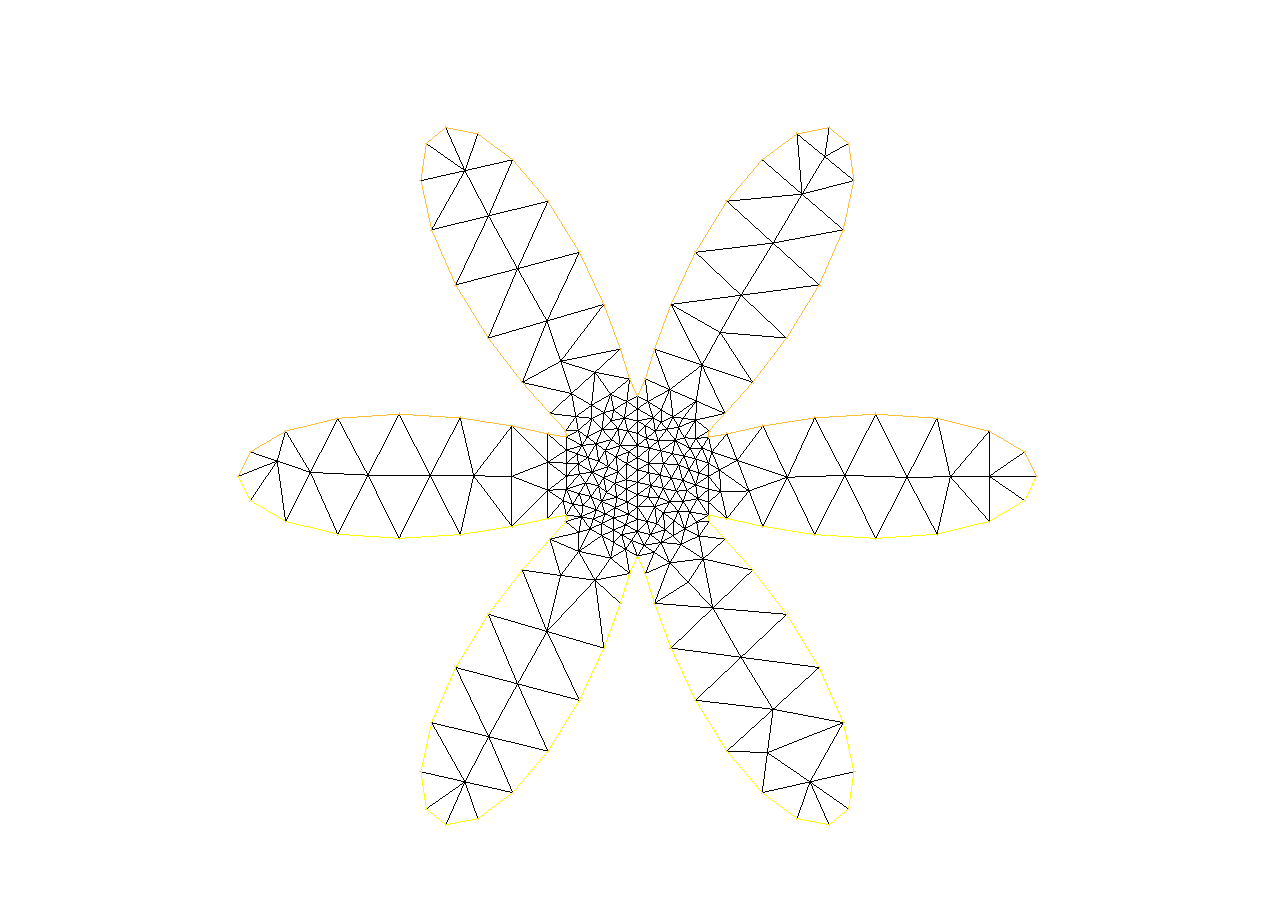
\includegraphics[width=0.9\linewidth]{picture/poisson2d}
		\caption{Mesh created by FreeFEM++ with division number=50}
		\label{fig:mesh}
	\end{subfigure}
	\quad
	\begin{subfigure}[b]{0.5\linewidth}
		\centering
		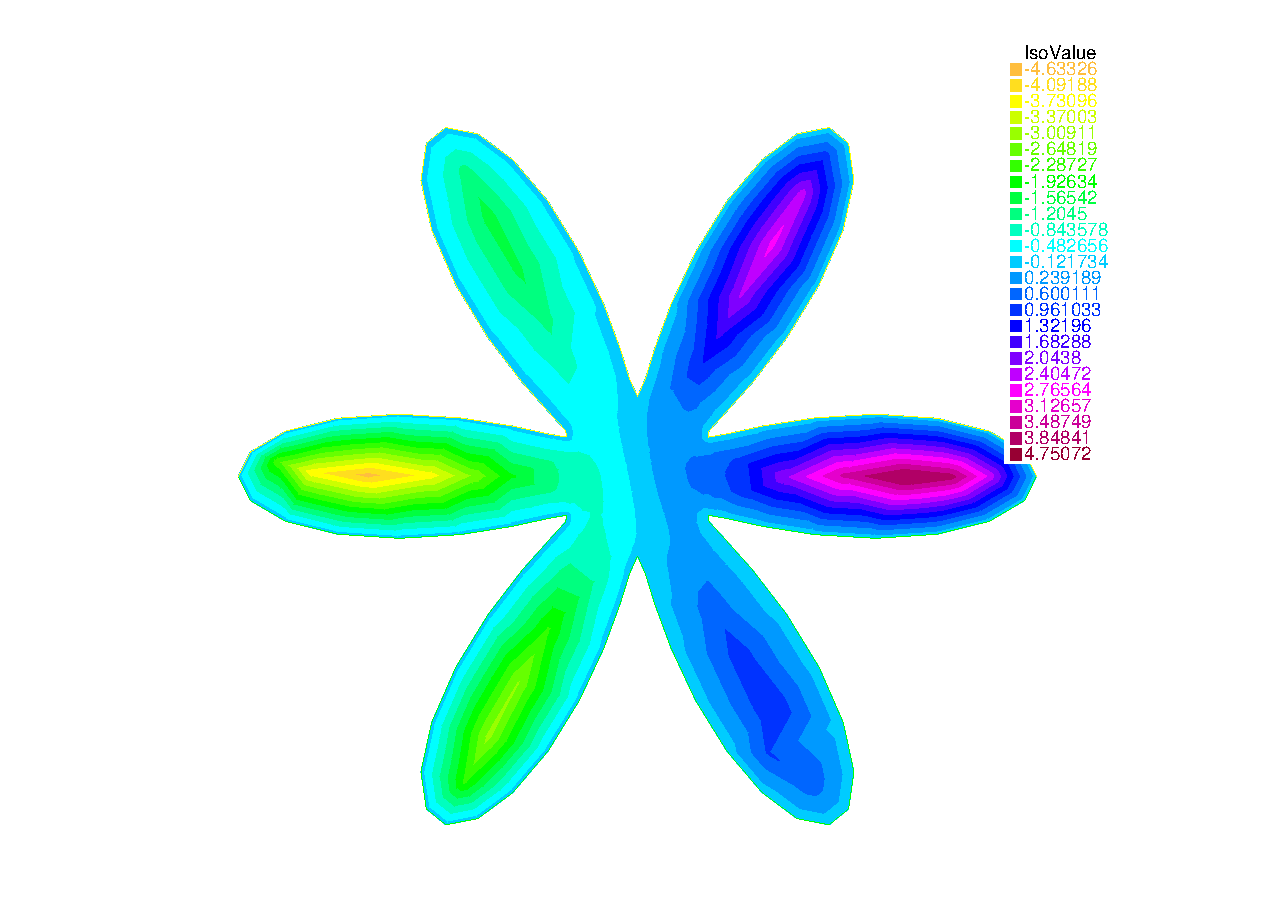
\includegraphics[width=0.9\linewidth]{picture/vectoru}
		\caption{Graphics of solution $u$ from 2D Poisson Problem, color palette on the right side show the value of $u$ on each point.}
		\label{fig:solution}
	\end{subfigure}
	\caption{The Mesh and Result of 2D Poisson Problem}
	\label{fig:result}
\end{figure}
\end{document}